\documentclass[12pt,a4paper,bibliography=totocnumbered]{scrartcl}
\usepackage[ngerman]{babel}

\usepackage{graphicx}
\usepackage{geometry}
%\usepackage{titlesec}
\usepackage{fancyhdr}
\usepackage[pdfpagelabels=true]{hyperref}
\usepackage{xcolor}
\usepackage{listings}
\usepackage[T1]{fontenc}

\definecolor{mGreen}{rgb}{0,0.6,0}
\definecolor{mGray}{rgb}{0.5,0.5,0.5}
\definecolor{airforceblue}{rgb}{0.36, 0.54, 0.66}
\definecolor{amber}{rgb}{1.0, 0.49, 0.0}
\definecolor{coolgrey}{rgb}{0.55, 0.57, 0.67}
\definecolor{davy}{rgb}{0.33, 0.33, 0.33}
\definecolor{backgroundColour}{rgb}{0.95,0.95,0.95}

\lstdefinestyle{CStyle}{
    backgroundcolor=\color{backgroundColour},   
    commentstyle=\color{davy},
    keywordstyle=\color{amber},
    numberstyle=\tiny\color{mGray},
    stringstyle=\color{airforceblue},
    basicstyle=\footnotesize,
    breakatwhitespace=false,         
    breaklines=true,                 
    captionpos=b,                    
    keepspaces=true,                 
    numbers=left,                    
    numbersep=5pt,                  
    showspaces=false,                
    showstringspaces=false,
    showtabs=false,                  
    tabsize=2,
    language=C
}

\geometry{a4paper, top=27mm, left=25mm, right=25mm, bottom=35mm, headsep=10mm, footskip=12mm}

\makeatletter
\renewcommand\@biblabel[1]{}
\makeatother
%__________________________________________________________________

\begin{document}

%\titlespacing{\section}{0pt}{12pt plus 4pt minus 2pt}{-6pt plus 2pt minus 2pt}

% Kopf- und Fusszeile
\pagestyle{fancy}
\renewcommand{\sectionmark}[1]{\markright{\arabic{section}.\ #1}}
\renewcommand{\leftmark}{}
\fancyhf{}
\lhead{}
\chead{}
\rhead{\thesection\space\contentsname}
\lfoot{Abgabe 1}
\cfoot{}
\rfoot{\ \linebreak  \thepage}
\renewcommand{\headrulewidth}{0.4pt}
\renewcommand{\footrulewidth}{0.4pt}

%______________________________________________________________________


%______________________________________________________________________

\clearpage

% Arabische Seitenzahlen
\pagenumbering{arabic}
\setcounter{page}{1}

% Geändertes Format für Seitenränder, arabische Seitenzahlen
\fancyhead[LE,RO]{\rightmark}
%\fancyhead[LO,RE]{\leftmark}
\fancyfoot[LE,RO]{\thepage}

%______________________________________________________________________

\section*{Abgabe 2}

\begin{lstlisting}[style=CStyle]
/*
 * This program calculates the time required to
 * execute the program specified as its first argument.
 * The time is printed in seconds, on standard out.
 */
#include <stdio.h>
#include <unistd.h>
#include <stdlib.h>
#include <time.h>
#include <sys/neutrino.h>

#define MILLISECONDS_PER_SECOND  1E6
#define TIME_TO_WAIT 1000000 //1ms

struct timespec rqtp, start, stop;

/*
 * Prints current frequency of system tick
 * Changes system tick to nanosecs
 * Prints new frequency of system tick
 * System tick indicates the frequency how oft the cpu is interrupted from the clock
 * Minimal value is 10 microseconds
 */
int changeSystemTick(unsigned int nanosecs) {

	struct _clockperiod new, old;

	if (ClockPeriod(CLOCK_REALTIME, NULL, &old, 0) != 0) {
		perror("clock period");
		return EXIT_FAILURE;
	}

	printf("old fract: %ld, old nsec: %ld \n", old.fract, old.nsec);

	new = old;
	new.nsec = nanosecs;

	if (ClockPeriod(CLOCK_REALTIME, &new, NULL, 0) != 0) {
		perror("clock period");
		return EXIT_FAILURE;
	}

	if (ClockPeriod(CLOCK_REALTIME, NULL, &old, 0) != 0) {
		perror("clock period");
		return EXIT_FAILURE;
	}

	printf("new fract: %ld, new nsec: %ld \n", old.fract, old.nsec);

	return EXIT_SUCCESS;
}

/* 
 * Simulates a cycle of TIME_TO_WAIT
 * Get current time with clock_gettime
 * For initialization setStart = 1
 * To simulate an ongoing cycle setStart = 0 for every iteration
 * Add TIME_TO_WAIT to the start time
 * With clock_nanosleep the programm sleeps until TIME_TO_WAIT is over
 */
int takt(int setStart) {
	int s;
	int ms;
	int err;

	if (clock_gettime(CLOCK_REALTIME, &start) == -1) {
		perror("clock gettime");
		return EXIT_FAILURE;
	}

	if (setStart == 1) {
		rqtp = start;
	}

	rqtp.tv_nsec += TIME_TO_WAIT;

	err = clock_nanosleep(CLOCK_REALTIME, TIMER_ABSTIME, &rqtp, NULL);
	if (err != 0) {
		printf("clock nanosleep: %d \n", strerror(err));
	}

	if (clock_gettime(CLOCK_REALTIME, &stop) == -1) {
		perror("clock gettime");
		return EXIT_FAILURE;
	}

	return EXIT_SUCCESS;
}

/*
 * Set system tick
 * Simulate ongoing cycle of 1ms
 * Print the waited miliseconds, check continuity of the results
 */
int main(int argc, char** argv) {
	changeSystemTick(1 * MILLISECONDS_PER_SECOND);
	int i = 0;
	takt(1);

	while(i < 20){
		takt(0);
		i++;
	}
	int s,ms;
	s = (stop.tv_sec - start.tv_sec) * 1000;
	ms = (stop.tv_nsec - start.tv_nsec) / MILLISECONDS_PER_SECOND;

	printf("start: %ld, n %ld \n", start.tv_sec, start.tv_nsec);
	printf("stop: %ld, n %ld \n", stop.tv_sec, stop.tv_nsec);
	printf("Waited miliseconds: %d\n", s + ms);
	return EXIT_SUCCESS;
}
\end{lstlisting}

\begin{figure}[h]
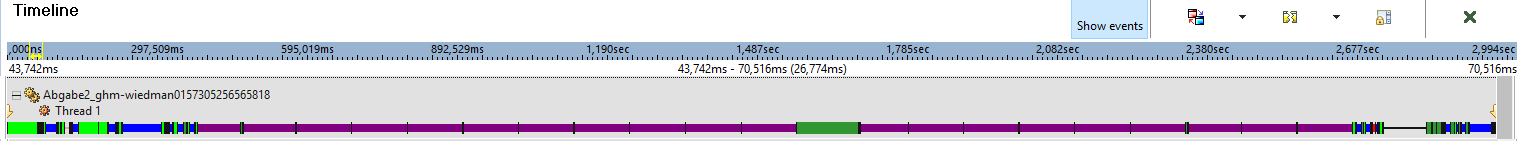
\includegraphics[width=\textwidth]{bilder/QNX_Abgabe2}
\centering
\end{figure}
Bei Überprüfung des Codes mit dem Kernel Event Tracer ist zu sehen, dass bei einer Durchführung mit System Takt mit >=1ms durch den simulierten Takt immer 1ms geschlafen wird.

\begin{figure}[h]
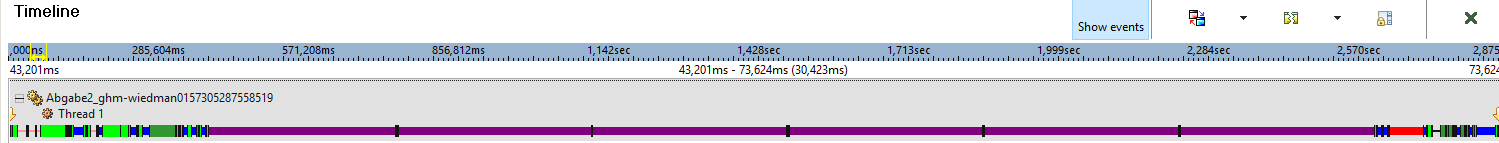
\includegraphics[width=\textwidth]{bilder/QNX_Abgabe2_4sec}
\centering
\end{figure}
Wenn der System Takt <1ms wird der simulierte Takt dem System Takt angepasst, da nur alle zb 4ms ein Interrupt durch den Sheduler passiert und das Programm nur bei einem Interrupt aufwachen kann.

\begin{figure}[h]
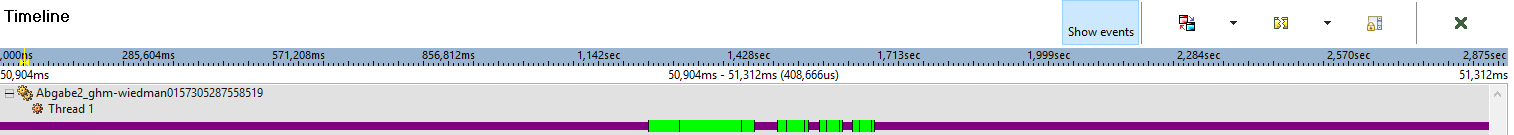
\includegraphics[width=\textwidth]{bilder/QNX_Abgabe2_4ticks}
\centering
\end{figure}
Da nur eine ms geschlafen hätte werden sollen, liegt die Aufwachszeit der nächsten x Iterationen in der Vergangenheit. Das heißt das Programm geht nur kurz in den sleep, wo dies dann bemerkt wird und er wieder aufwacht.

%______________________________________________________________________

\end{document}












